\documentclass[11pt,a4paper]{article}
\usepackage[left=23mm,right=23mm,top=22mm,bottom=22mm,footskip=11mm]{geometry}
\usepackage{amsmath,amssymb}
\usepackage{assets/tex/cm-bea}
\usepackage{xeCJK}
\setmainfont{Latin Modern Roman}
\setCJKmainfont{FandolSong-Regular.otf}[Path=assets/fonts/fandol/,BoldFont=FandolSong-Bold.otf,ItalicFont=FandolSong-Regular.otf]
\setCJKsansfont{FandolSong-Regular.otf}[Path=assets/fonts/fandol/,BoldFont=FandolSong-Bold.otf]
\renewcommand{\bfdefault}{bx}
\xeCJKsetup{PunctStyle=quanjiao,CheckSingle=true}
\usepackage{setspace}\setstretch{1.10}
\setlength{\parindent}{2em}\setlength{\parskip}{4pt}
\usepackage{xcolor,titlesec,tikz,enumitem,longtable,booktabs,array,calc,needspace}
\usepackage{assets/tex/s-style-boxes}
\usetikzlibrary{arrows.meta,positioning}
\definecolor{sitepaper}{HTML}{FFFEFC}\pagecolor{sitepaper}
\definecolor{navy}{HTML}{10136B}\definecolor{warm}{HTML}{94662C}
\titleformat{\section}{\Large\bfseries\color{navy}}{}{0pt}{}
\titleformat{\subsection}{\normalsize\bfseries\color{navy}}{}{0pt}{}
\titlespacing*{\section}{0pt}{17pt}{9pt}\titlespacing*{\subsection}{0pt}{12pt}{6pt}
\setlist[enumerate]{leftmargin=2.2em,itemsep=3pt,parsep=0pt,topsep=3pt}
\setlist[itemize]{label={},leftmargin=1em,itemsep=3pt}
\providecommand{\tightlist}{\setlength{\itemsep}{3pt}\setlength{\parskip}{0pt}}
\usepackage[unicode,hidelinks,linktoc=all]{hyperref}\usepackage{bookmark}
\hypersetup{pdftitle={正交多项式的性质与经典应用},pdfauthor={Vincent Arqain}}
\renewcommand{\contentsname}{目录}\setcounter{tocdepth}{1}\setcounter{secnumdepth}{0}
\widowpenalty=10000\clubpenalty=10000\displaywidowpenalty=10000\predisplaypenalty=5000
\allowdisplaybreaks[1]\raggedbottom\emergencystretch=2em

\newcommand{\lectureheading}[1]{\section{#1}}
\newcommand{\lecturerule}{\par\noindent{\color{navy!48}\rule{\linewidth}{0.45pt}}\par}


\begin{document}

\begin{center}{\LARGE\bfseries 正交多项式的性质与经典应用\par}\vspace{6pt}{\large 从正交投影、零点交错到最优求积\par}\end{center}

给定四次函数 \(x^4\)，怎样用次数不超过三的多项式来近似它？在 \([-1,1]\) 上，平衡总平方误差与压低最大误差，会得到两个不同的答案。前者用 Legendre 多项式，后者用第一类 Chebyshev 多项式。§5 将把两条误差曲线画在同一组坐标轴上。

本讲以《函数逼近：思路与方法》§4 为中心，衔接原稿 §2 的一致逼近、§3 的平方逼近和 §5 的离散拟合。记 \(\mathcal P_n\) 为次数不超过 \(n\) 的实多项式空间，\(\mathcal P_{-1}=\{0\}\)。``首一''指最高次项系数为 \(1\)。

\medskip\noindent{\large\bfseries\color{navy} 五族多项式与它们的用途}

\begin{center}\small\setlength{\tabcolsep}{4pt}\renewcommand{\arraystretch}{1.27}
\begin{tabular}{@{}p{.195\linewidth}p{.18\linewidth}p{.279\linewidth}p{.275\linewidth}@{}}\toprule
多项式 & 区间与权函数 & 决定应用的性质 & 本讲中的应用 \\ \midrule
Legendre \(P_n\) & \([-1,1]\)，\(1\) & 单位端点值，平方范数 \(\frac{2}{2n+1}\) & 绝对值函数的投影、等权 Gauss 求积 \\
Chebyshev \(T_n\) & \([-1,1]\)，\((1-x^2)^{-\frac{1}{2}}\) & 等幅交错，首一形式最大模最小 & 多项式降阶、插值节点选择 \\
Chebyshev \(U_n\) & \([-1,1]\)，\((1-x^2)^{\frac{1}{2}}\) & 正弦表示给出全部零点 & 固定端振动链的模态 \\
Laguerre \(\ell_n\) & \([0,\infty)\)，\(e^{-x}\) & Rodrigues 公式将投影系数化为指数矩 & 衰减函数的展开及误差 \\
Hermite \(H_n\) & \(\mathbb R\)，\(e^{-x^2}\) & 导数降低次数，高斯因子给出正交特征函数 & 一维谐振子 \\ \bottomrule\end{tabular}\end{center}

\begingroup\small\setlength{\parskip}{1pt}\tableofcontents\endgroup

\clearpage\lectureheading{§1 从正交化到最佳平方逼近}

设 \(I=(a,b)\)，端点可为无穷。设权函数 \(w\) 几乎处处为正，且对每个非负整数 \(k\) 有 \(\int_I |x|^k w(x)\,dx<\infty\)。在实函数上记

\[
\langle f,g\rangle_w=\int_I f(x)g(x)w(x)\,dx,\qquad
\|f\|_w^2=\langle f,f\rangle_w .
\]

非零多项式只有有限个零点，故其平方范数严格为正。从 \(1,x,x^2,\ldots\) 出发，逐次减去低次方向上的分量，便能留下一个仍然首一、但与所有低次多项式正交的多项式。

\begin{sboxenv}{navy}{性质 1.1　每个次数恰有一个首一正交多项式}

记它为 \(\pi_n\)，令 \(h_n=\|\pi_n\|_w^2\)。从 \(\pi_0=1\) 起有

\[
\pi_n(x)=x^n-\sum_{j=0}^{n-1}
\frac{\langle x^n,\pi_j\rangle_w}{h_j}\,\pi_j(x).
\]

\end{sboxenv}

\textbf{证明}　右边的最高次项为 \(x^n\)。分别与 \(\pi_0,\ldots,\pi_{n-1}\) 作内积，各次投影恰好抵消。由于次数不同，这 \(n\) 个多项式构成 \(\mathcal P_{n-1}\) 的基。若另有一个首一解，两解之差既属于 \(\mathcal P_{n-1}\) 又与它正交，因而范数为零，两解相同。

\begin{sboxenv}{navy}{定理 1.2　正交投影与误差恒等式}

对 \(f\in L^2(I,w\,dx)\)，取任意按次数排列的正交基 \(p_j\)，记 \(d_j=\|p_j\|_w^2\)。在 \(\mathcal P_m\) 中唯一的最佳平方逼近为

\[
S_m f=\sum_{j=0}^m c_jp_j,\qquad c_j=\frac{\langle f,p_j\rangle_w}{d_j}.
\]

对所有 \(q\in\mathcal P_m\)，有 \(\|f-q\|_w^2=\|f-S_m f\|_w^2+\|S_m f-q\|_w^2\)。

\end{sboxenv}

\textbf{证明}　按系数定义，残差 \(f-S_m f\) 与每个 \(p_j\)（\(0\le j\le m\)）正交。将 \(f-q=(f-S_m f)+(S_m f-q)\) 展开平方，交叉项为零。最后一项只在 \(q=S_m f\) 时为零。取 \(q=0\) 还得到

\[
\|f-S_m f\|_w^2=\|f\|_w^2-\sum_{j=0}^m c_j^2 d_j .
\]

右端非负即 Bessel 不等式。随着 \(m\) 增大，每增加一项，平方误差恰好减少 \(c_{m+1}^2 d_{m+1}\)。若多项式在相应 \(L^2\) 空间中稠密，最佳误差趋于零，取极限便得到 Parseval 等式。在有限闭区间的连续函数情形，Weierstrass 定理给出一致逼近，再用 \(\|g\|_w\le\sqrt{\int_I w}\,\|g\|_\infty\) 即可。

\textbf{首一极小性}　任意首一 \(n\) 次多项式唯一写成 \(\pi_n+r\)，其中 \(r\in\mathcal P_{n-1}\)。正交性给出 \(\|\pi_n+r\|_w^2=h_n+\|r\|_w^2\)。求 \(x^n\) 的最佳低一阶逼近时，因此只需从 \(x^n\) 减去 \(\pi_n\)。

\clearpage\lectureheading{§2 三项递推与零点交错}

构造 \(\pi_{n+1}\) 时，本来需要减去沿所有低次基向量的投影。改从 \(x\pi_n\) 开始，就能利用乘以 \(x\) 的对称性，把需要计算的投影压缩到两个。

\begin{sboxenv}{navy}{定理 2.1　三项递推}

\(\pi_1=x-\alpha_0\)。当 \(n\ge1\) 时，

\[
\begin{aligned}
\pi_{n+1}&=(x-\alpha_n)\pi_n-\beta_n\pi_{n-1},\\
\alpha_n&=\frac{\langle x\pi_n,\pi_n\rangle_w}{h_n},
&\beta_n&=\frac{h_n}{h_{n-1}}>0 .
\end{aligned}
\]

\end{sboxenv}

\textbf{证明}　展开 \(x\pi_n\)。它首一，故 \(\pi_{n+1}\) 的系数为 \(1\)。若 \(j\le n-2\)，则 \(\langle x\pi_n,\pi_j\rangle_w=\langle\pi_n,x\pi_j\rangle_w=0\)。而 \(x\pi_{n-1}-\pi_n\) 次数小于 \(n\)，故 \(\langle x\pi_n,\pi_{n-1}\rangle_w=h_n\)。除以对应平方范数即得两系数。在关于原点对称的区间上，若 \(w\) 为偶函数，则 \((-1)^n\pi_n(-x)\) 满足同一首一正交条件，故 \(\pi_n\) 与 \(n\) 同奇偶，且 \(\alpha_n=0\)。

\begin{sboxenv}{navy}{定理 2.2　单零点与严格交错}

\(\pi_n\) 在 \((a,b)\) 有 \(n\) 个互异的单零点。设其零点为 \(r_1<\cdots<r_n\)，则 \(\pi_{n+1}\) 的 \(n+1\) 个零点在由这些点分成的 \(n+1\) 个开区间中各占一个。

\end{sboxenv}

\textbf{证明}　把 \(\pi_n\) 在 \((a,b)\) 内所有变号点记为 \(t_1,\ldots,t_s\)。若 \(s<n\)，令 \(q(x)=\prod_{i=1}^{s}(x-t_i)\)（空积为 \(1\)）。积 \(\pi_n q\) 在整个区间不变号，且仅在有限个点为零，于是其加权积分非零。这与 \(q\in\mathcal P_{n-1}\) 矛盾。因此 \(s=n\)，次数已经用尽，这些根均为单根。

用递推证明交错。归纳假定 \(\pi_{n-1}\) 的零点各落在相邻 \(r_i\) 之间。代入 \(r_i\) 得 \(\pi_{n+1}(r_i)=-\beta_n\pi_{n-1}(r_i)\)，这些值依次异号，故每个内部间隙都有根。由于首一，\(\pi_{n-1}(r_n)>0\)，而 \(\pi_{n+1}\) 在充分大的正数处为正，右侧还有一根。左端同理，\(\pi_{n+1}(r_1)\) 的符号为 \((-1)^n\)，与其在充分小的负数处的符号相反。上段已保证所有根都在 \((a,b)\) 内。\(n=1\) 时取 \(\pi_0=1\)，同一端点论证即给出归纳起点。

\textbf{为何要控制零点}　将这 \(n\) 个点用作积分节点，任意 \(\pi_n q\) 在全部节点上的函数值均为零。只要 \(\deg q<n\)，它的积分也因正交性为零。§9 正是利用这两种``为零''把求积精度提高到 \(2n-1\) 次。

\textbf{Christoffel--Darboux 公式。} 取 \(K_m(x,y)=\sum_{j=0}^m\frac{\pi_j(x)\pi_j(y)}{h_j}\)。对 \(x\ne y\) 有

\[
K_m(x,y)=\frac{\pi_{m+1}(x)\pi_m(y)-\pi_m(x)\pi_{m+1}(y)}
{h_m(x-y)} .
\]

\textbf{证明}　记 \(D_j=\pi_{j+1}(x)\pi_j(y)-\pi_j(x)\pi_{j+1}(y)\)。在 \(x,y\) 写出三项递推，分别乘以 \(\pi_j(y),\pi_j(x)\) 再相减，得 \((x-y)\pi_j(x)\pi_j(y)=D_j-\beta_jD_{j-1}\)。除以 \(h_j\)，利用 \(\frac{\beta_j}{h_j}=\frac{1}{h_{j-1}}\)，从 \(j=0\) 累加，中间项全部抵消（首项取 \(D_{-1}=0\)）。这给出只用相邻两阶计算整个和式的办法。由逐项积分，对每个 \(q\in\mathcal P_m\) 都有 \(\int_I K_m(x,y)q(y)w(y)\,dy=q(x)\)。§10 将用这一性质直接计算求积权重。

\clearpage\lectureheading{§3 Legendre 多项式与平均平方误差}

在 \([-1,1]\) 上取 \(w=1\)。采用 \(P_n(1)=1\) 的归一化。Rodrigues 公式的意义在于，分部积分 \(n\) 次后，导数全部转移到待检验的多项式上。

\begin{sboxenv}{navy}{性质 3.1　Rodrigues 公式、范数与递推}

\[
P_n(x)=\frac{1}{2^n n!}\frac{d^n}{dx^n}(x^2-1)^n,\qquad
\int_{-1}^1 P_n^2\,dx=\frac{2}{2n+1}.
\]

\(P_0=1,\ P_1=x\)。对 \(n\ge1\)，

\[
(n+1)P_{n+1}=(2n+1)xP_n-nP_{n-1}.
\]

\end{sboxenv}

\textbf{证明}　\((x^2-1)^n\) 在两端有 \(n\) 重零点，所以分部积分不留边界项。对 \(\deg q<n\)，\(q^{(n)}=0\)，故 \(\int_{-1}^1 P_nq=0\)。在 \(x=1\) 对 \((x-1)^n(x+1)^n\) 求 \(n\) 阶导数，只有全部求导作用在第一因子上的一项保留，给出 \(P_n(1)=1\)。首项系数为 \(k_n=2^{-n}\binom{2n}{n}\)。由奇偶性和定理 2.1，\(xP_n=A_nP_{n+1}+B_nP_{n-1}\)。比较首项得 \(A_n=\frac{k_n}{k_{n+1}}=\frac{n+1}{2n+1}\)，代入 \(x=1\) 得 \(B_n=\frac{n}{2n+1}\)。以 \(d_n=\|P_n\|^2\) 记范数平方，比较 \(\langle xP_{n-1},P_n\rangle\) 与 \(\langle P_{n-1},xP_n\rangle\) 得 \(d_n=\frac{(2n-1)d_{n-1}}{2n+1}\)。从 \(d_0=2\) 连乘便得结论。

\begin{sboxenv}{orange}{例 1　用二次多项式逼近绝对值函数}

求 \(f(x)=|x|\) 在 \([-1,1]\) 上的最佳平方逼近 \(S_2 f\)，并计算最小平方误差。

\end{sboxenv}

\textbf{解}　\(P_2=\frac{3x^2-1}{2}\)。由奇偶性，\(P_1\) 项为零，只需两个积分。因为 \(\int_{-1}^1|x|\,dx=1\)，而 \(\int_{-1}^1|x|P_2(x)\,dx=\int_0^1 x(3x^2-1)\,dx=\frac{1}{4}\)，所以

\[
\begin{aligned}
S_2 f&=\frac12P_0+\frac58P_2=\frac{15x^2+3}{16},\\
\|f-S_2 f\|_2^2
&=\frac23-2\left(\frac12\right)^2-\frac25\left(\frac58\right)^2
=\frac{1}{96}.
\end{aligned}
\]

这说明近似多项式可以在 \(x=0\) 取 \(\frac{3}{16}\)，即使原函数在此为零。决定系数的条件是残差对 \(1,x,x^2\) 的三个积分均为零。在一般有限区间 \([a,b]\) 上，用 \(t=\frac{2x-a-b}{b-a}\) 将 \(P_j(t)\) 移到新区间。积分中的公共常数 \(\frac{b-a}{2}\) 在计算投影系数时约去。

\textbf{微分方程与球面上的轴对称模式。} 定义 \(Au=-[(1-x^2)u']'\)。因端点因子为零，两次分部积分给出 \(\langle AP_n,q\rangle=\langle P_n,Aq\rangle\)。而 \(A\) 将 \(\mathcal P_{n-1}\) 映入自身，故 \(AP_n\) 也与该空间正交。比较 \(x^n\) 的系数知

\[
-\bigl[(1-x^2)P_n'(x)\bigr]'=n(n+1)P_n(x).
\]

这解释了同一族多项式为何出现在球面上。令极角为 \(\theta\)，轴对称函数写成 \(v(\theta)=P_n(\cos\theta)\)。代入球面角向算子 \(-(\sin\theta)^{-1}(\frac{d}{d\theta})(\sin\theta\,\frac{dv}{d\theta})\)，取 \(x=\cos\theta\) 后恰得到 \(AP_n\)。于是常数、\(\cos\theta\) 和 \(\frac{3\cos^2\theta-1}{2}\) 分别对应特征值 \(0,2,6\)。

\clearpage\lectureheading{§4 第一类 Chebyshev 多项式与极小偏差}

令 \(x=\cos\theta\)，\(0\le\theta\le\pi\)，取 \(T_n(\cos\theta)=\cos(n\theta)\)。余弦加法公式立即给出 \(T_0=1,\ T_1=x,\ T_{n+1}=2xT_n-T_{n-1}\)，故 \(T_n\) 确是多项式。当 \(n\ge1\) 时，它的首项系数为 \(2^{n-1}\)，与 \(n\) 同奇偶。变量代换把带有端点奇性的权变成了均匀的角度测度：

\[
\int_{-1}^1\frac{T_m(x)T_n(x)}{\sqrt{1-x^2}}\,dx
=\int_0^\pi\cos(m\theta)\cos(n\theta)\,d\theta .
\]

积化和差给出 \(m\ne n\) 时积分为零。平方范数在 \(n=0\) 时为 \(\pi\)，在 \(n\ge1\) 时为 \(\frac{\pi}{2}\)。因此这族多项式的\textbf{正交性}来自余弦函数的正交，而下面的\textbf{一致极小性}另有依据，即相邻极值之间的等幅振荡。

\begin{sboxenv}{navy}{定理 4.1　首一多项式的最小最大模}

对 \(n\ge1\)，令 \(C_n=2^{1-n}T_n\)。在 \([-1,1]\) 上的所有首一 \(n\) 次多项式中，\(C_n\) 唯一使最大模最小，最小值为 \(E=2^{1-n}\)。

\end{sboxenv}

\textbf{证明}　取递增极值点 \(y_j=-\cos(\frac{j\pi}{n})\)，\(0\le j\le n\)。有 \(C_n(y_j)=(-1)^{n-j}E\)，且 \(\|C_n\|_\infty=E\)。若另一个首一多项式 \(p\) 满足 \(\|p\|_\infty\le E\)，记 \(d=C_n-p\)，则 \(\deg d\le n-1\)，每个 \((-1)^{n-j}d(y_j)\ge0\)。在这 \(n+1\) 个点上对 \(d\) 作 Lagrange 插值，比较 \(x^n\) 的系数得

\[
0=\sum_{j=0}^{n}\frac{d(y_j)}{\prod_{i\ne j}(y_j-y_i)} .
\]

各分母的符号恰为 \((-1)^{n-j}\)，故各项均非负，只能全部为零。于是 \(d\) 有 \(n+1\) 个零点，必恒为零。这个论证也处理了某些极值点处两个多项式恰好相等的情形。

\begin{sboxenv}{orange}{例 2　如何选择插值节点}

对 \(f\in C^{n+1}[-1,1]\) 作 \(n\) 次插值。若只知道 \(\|f^{(n+1)}\|_\infty\le M\)，怎样选择 \(n+1\) 个节点，使经典余项给出的统一上界最小？

\end{sboxenv}

\textbf{解}　对互异节点 \(x_0,\ldots,x_n\) 记 \(\omega(x)=\prod_{j=0}^n(x-x_j)\)。在非节点 \(x\)，从 \(f-I_nf\) 减去适当倍数的 \(\omega\)，使差在 \(x\) 也消失。对这 \(n+2\) 个零点反复用 Rolle 定理，得

\[
f(x)-I_nf(x)=\frac{f^{(n+1)}(\xi_x)}{(n+1)!}\,\omega(x).
\]

节点处误差本身为零。因 \(\omega\) 首一，定理 4.1 给出最优节点多项式 \(2^{-n}T_{n+1}\)。解 \(\cos((n+1)\theta)=0\) 得

\[
x_j=\cos\frac{(2j+1)\pi}{2(n+1)},\quad 0\le j\le n,\qquad
\|f-I_nf\|_\infty\le\frac{M}{2^n(n+1)!}.
\]

取 \(f(x)=\frac{Mx^{n+1}}{(n+1)!}\) 即取等号，所以这个函数类上的最坏误差界也是精确的。对一个指定的 \(f\)，最优节点还可能利用它自身的信息。映射到 \([a,b]\) 后，节点多项式的最大模另乘 \((\frac{b-a}{2})^{n+1}\)。

\clearpage\lectureheading{§5 同题对照：把四次函数降阶}

\begin{sboxenv}{orange}{例 3　在两种误差准则下逼近同一个函数}

令 \(f(x)=x^4\)，\(-1\le x\le1\)。在 \(\mathcal P_3\) 中分别求使 \(\int_{-1}^1|f-q|^2\,dx\) 最小和使 \(\max_{[-1,1]}|f-q|\) 最小的多项式。

\end{sboxenv}

\textbf{解}　无论选哪个 \(q\)，残差 \(x^4-q\) 都是首一四次多项式，反之每个首一四次多项式都是一个候选残差。因而所求的两个残差可以直接从 §1 与 §4 的极小性质读出。由递推式得到

\[
P_4(x)=\frac{35x^4-30x^2+3}{8},\qquad T_4(x)=8x^4-8x^2+1 .
\]

\textbf{平方误差最小。} 把 \(P_4\) 化为首一，得 \(r_2=\frac{8}{35}P_4\)，故 \(q_2=\frac{6}{7}x^2-\frac{3}{35}\)。残差对 \(1,x,x^2,x^3\) 都正交。最小平方误差为 \(\left(\frac{8}{35}\right)^2\frac{2}{9}=\frac{128}{11025}\)。

\textbf{最大误差最小。} 把 \(T_4\) 化为首一，得 \(r_\infty=\frac{T_4}{8}\)，故 \(q_\infty=x^2-\frac{1}{8}\)。在 \(-1,-\frac{1}{\sqrt2},0,\frac{1}{\sqrt2},1\) 上，残差依次取 \(\frac{1}{8},-\frac{1}{8},\frac{1}{8},-\frac{1}{8},\frac{1}{8}\)，故最小最大误差为 \(\frac{1}{8}\)。

\begin{center}

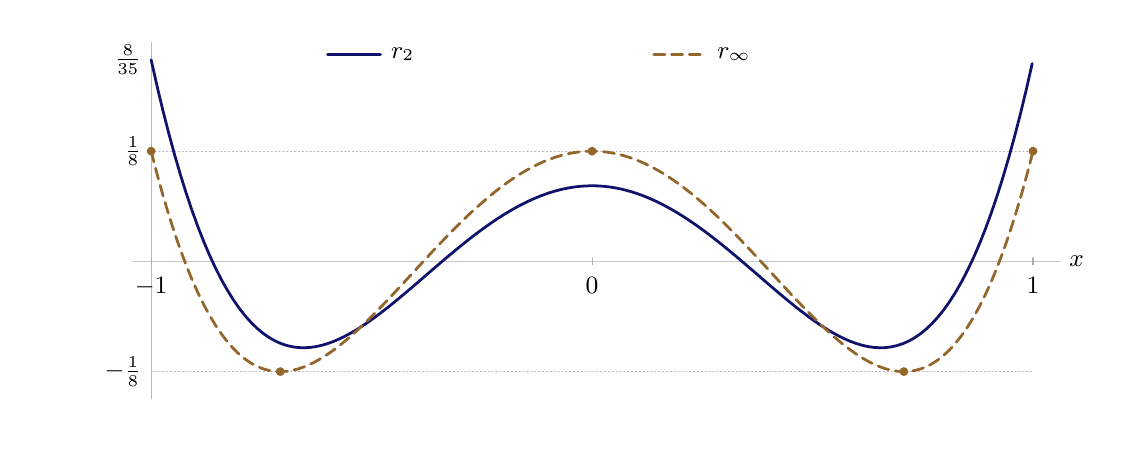
\begin{tikzpicture}[x=5.6cm,y=11.2cm,line cap=round,line join=round,font=\small]
  \path[use as bounding box] (-1.28,-.185) rectangle (1.18,.265);
  \draw[gray!45,thin] (-1.04,0)--(1.06,0) node[right,black] {$x$};
  \foreach \y in {-.125,.125}
    \draw[gray!55,thin,densely dotted] (-1,\y)--(1,\y);
  \draw[gray!55,thin] (-1,-.156)--(-1,.248);
  \foreach \x/\txt in {-1/-1,0/0,1/1}
    \draw[gray!65] (\x,.004)--(\x,-.004) node[below=1pt,black] {$\txt$};
  \node[left] at (-1,.22857) {$\frac{8}{35}$};
  \node[left] at (-1,.125) {$\frac18$};
  \node[left] at (-1,-.125) {$-\frac18$};
  \draw[color=navy,line width=1.0pt] plot[domain=-1:1,samples=151] (\x,{(\x)*(\x)*(\x)*(\x)-6*(\x)*(\x)/7+3/35});
  \draw[color=warm,line width=1.0pt,dash pattern=on 4pt off 2.4pt] plot[domain=-1:1,samples=151] (\x,{(\x)*(\x)*(\x)*(\x)-(\x)*(\x)+1/8});
  \foreach \x/\y in {-1/.125,-.7071068/-.125,0/.125,.7071068/-.125,1/.125}
    \fill[warm] (\x,\y) circle[radius=1.6pt];
  \draw[navy,line width=1pt] (-.60,.235)--(-.48,.235) node[right,black] {$r_2$};
  \draw[warm,line width=1pt,dash pattern=on 4pt off 2.4pt] (.14,.235)--(.26,.235) node[right,black] {$r_\infty$};
\end{tikzpicture}


\end{center}

图 1　实线为平方误差最小的残差，虚线为最大误差最小的残差。前者在两端升到 \(\frac{8}{35}\)，后者将五个峰谷的绝对值压到同一高度。还可以直接算出 \(\int_{-1}^1r_\infty^2\,dx=\frac{31}{2016}>\frac{128}{11025}\)，核对两种极小性质。

\textbf{降阶的一般式。} 若 \(F\) 为 \(n\) 次多项式、首项系数为 \(a_n\)，则在 \(\mathcal P_{n-1}\) 中的最佳一致逼近为 \(F-a_n2^{1-n}T_n\)。确切的最小最大误差是 \(|a_n|2^{1-n}\)。最佳平方逼近同样由 \(F-a_n\pi_n\) 给出，其中 \(\pi_n\) 须按指定权函数构造。一次降低一阶时，这两个结论都给出精确解。

\textbf{展开截断、节点插值和最佳一致逼近。} 对 \(T_n\) 作带权正交展开，截断得到的是该权下的最佳平方逼近。取 \(f(x)=|x|\)，只允许保留常数项，三种操作已经给出三个结果。投影系数是 \(\pi^{-1}\int_0^\pi|\cos\theta|\,d\theta=\frac{2}{\pi}\)。单点 Chebyshev 插值取 \(T_1\) 的零点 \(0\)，故插值常数为 \(0\)。最佳一致常数则使 \(|c|\) 与 \(|1-c|\) 平衡，取 \(c=\frac{1}{2}\)。单靠基函数名称不足以确定所求的近似。

\clearpage\lectureheading{§6 第二类 Chebyshev 多项式与振动模态}

对 \(0<\theta<\pi\)，令 \(U_n(\cos\theta)=\frac{\sin((n+1)\theta)}{\sin\theta}\)。正弦加法公式给出 \(U_0=1,\ U_1=2x,\ U_{n+1}=2xU_n-U_{n-1}\)。故首项系数为 \(2^n\)，两端可连续补为 \(U_n(1)=n+1\) 和 \(U_n(-1)=(-1)^n(n+1)\)。对 \(T_{n+1}(\cos\theta)\) 求导还得到 \(T_{n+1}'=(n+1)U_n\)。因此 \(U_n\) 的零点恰是 \(T_{n+1}\) 的内部极值点。

\begin{sboxenv}{navy}{性质 6.1　两类 Chebyshev 多项式所用的权}

第一类用 \(\frac{1}{\sqrt{1-x^2}}\)，第二类用 \(\sqrt{1-x^2}\)。第二类的 \(n\) 个零点为 \(\cos(\frac{k\pi}{n+1})\)，\(1\le k\le n\)，各阶平方范数均为 \(\frac{\pi}{2}\)。

\end{sboxenv}

\textbf{证明}　零点从正弦分子读出。代换 \(x=\cos\theta\) 后，权与微分贡献 \(\sin^2\theta\,d\theta\)，恰好约去两个 \(U\) 的分母。因此内积变成 \(\int_0^\pi\sin((m+1)\theta)\sin((n+1)\theta)\,d\theta\)，积化和差即证。两个权的差别反映出构造中是余弦本身，还是带分母的正弦。

\begin{sboxenv}{orange}{例 4　两端固定的离散振动链}

取 \(N\) 个内部点，补边界 \(v_0=v_{N+1}=0\)。定义 \((Kv)_j=2v_j-v_{j-1}-v_{j+1}\)，\(1\le j\le N\)。求所有振动模态，即 \(K\) 的特征值与特征向量。

\end{sboxenv}

\textbf{解}　将特征方程写成 \(v_{j+1}=(2-\lambda)v_j-v_{j-1}\)。非零向量必有 \(v_1\ne0\)，否则递推给出全零。令 \(v_1=1\)，置 \(t=1-\frac{\lambda}{2}\)，则 \(v_j=U_{j-1}(t)\)。右端边界要求 \(U_N(t)=0\)。于是

\[
\lambda_k=2-2\cos\frac{k\pi}{N+1},\qquad
v_j^{(k)}=\sin\frac{jk\pi}{N+1},\qquad 1\le k,j\le N ,
\]

其中向量已作常数倍调整。\(N\) 个特征值各不相同，给出了全部模态。以 \(N=2\) 检查，特征值为 \(1,3\)，特征方向分别为 \((1,1)\) 与 \((1,-1)\)。在单位质量、单位弹簧刚度的方程 \(\ddot v+Kv=0\) 中，两种角频率因而为 \(1\) 与 \(\sqrt3\)。

\textbf{同一组角度也给出第二类 Gauss--Chebyshev 求积。} 写 \(\theta_k=\frac{k\pi}{n+1}\)，\(z_k=\cos\theta_k\)，\(1\le k\le n\)。由定理 9.1，这些 \(U_n\) 的零点是权 \(\sqrt{1-x^2}\) 的 Gauss 节点。相应权重为 \(\lambda_k=\frac{\pi\sin^2\theta_k}{n+1}\)。验证时只需在基 \(U_0,\ldots,U_{n-1}\) 上核对。离散正弦正交给出

\[
\sum_{k=1}^n\sin\theta_k\sin((j+1)\theta_k)
=\begin{cases}\frac{n+1}{2},&j=0,\\0,&1\le j<n.\end{cases}
\]

对 \(j>0\)，两组正弦向量是上例中实对称矩阵的不同特征向量，故内积为零。对 \(j=0\)，用 \(\sin^2\theta=\frac{1-\cos 2\theta}{2}\) 及单位根之和即得。将上式乘以 \(\frac{\pi}{n+1}\)，结果与 \(\int_{-1}^1 U_j(x)\sqrt{1-x^2}\,dx\) 相同，因而权重正确。

\clearpage\lectureheading{§7 Laguerre 多项式与半轴上的指数逼近}

在 \([0,\infty)\) 上取 \(w(x)=e^{-x}\)。为便于同原稿核对，下文用 \(\ell_n\) 表示在原点取 \(1\) 的常用归一化，用 \(\mathcal L_n=n!\ell_n\) 表示原稿 §4.3 的记号。前几项为 \(\ell_0=1,\ \ell_1=1-x,\ \ell_2=1-2x+\frac{x^2}{2}\)。

\begin{sboxenv}{navy}{性质 7.1　Rodrigues 公式及归一化换算}

\[
\ell_n(x)=\frac{e^x}{n!}\frac{d^n}{dx^n}(x^n e^{-x})
=\sum_{j=0}^n(-1)^j\binom nj\frac{x^j}{j!}.
\]

\(\|\ell_n\|_w^2=1\)，\(\|\mathcal L_n\|_w^2=(n!)^2\)。对 \(n\ge1\)，两种递推分别为

\[
\begin{aligned}
(n+1)\ell_{n+1}&=(2n+1-x)\ell_n-n\ell_{n-1},\\
\mathcal L_{n+1}&=(2n+1-x)\mathcal L_n-n^2\mathcal L_{n-1}.
\end{aligned}
\]

\end{sboxenv}

\textbf{证明}　Leibniz 求导公式给出有限和。对多项式 \(q\)，把导数从 \(x^ne^{-x}\) 转移到 \(q\)。原点处有 \(n\) 重零点，无穷远处的多项式乘指数因子趋于零，故

\[
\langle q,\ell_n\rangle_w=\frac{(-1)^n}{n!}
\int_0^\infty q^{(n)}(x)x^n e^{-x}\,dx .
\]

取 \(\deg q<n\) 得正交。取 \(q=\ell_n\)，注意 \(\ell_n^{(n)}=(-1)^n\)，而 \(\int_0^\infty x^ne^{-x}\,dx=n!\)，得到单位范数。再展开 \(x\ell_n\)，定理 2.1 只留下三项。比较首项得 \(\ell_{n+1}\) 的系数 \(-(n+1)\)，由内积对称及单位范数知 \(\ell_{n-1}\) 的系数为 \(-n\)。在 \(x=0\) 代值，三个系数和为零，故中间系数为 \(2n+1\)。将递推乘以 \(n!\) 即得原稿形式。

从显式系数还可读出微分方程。若 \(\ell_n=\sum a_jx^j\)，则 \((j+1)^2a_{j+1}=-(n-j)a_j\)（令 \(a_{n+1}=0\)）。逐次比较系数即得 \(x\ell_n''+(1-x)\ell_n'+n\ell_n=0\)。乘以 \(e^{-x}\) 可写成 \(-(xe^{-x}\ell_n')'=ne^{-x}\ell_n\)，其右端的权正与定义一致。

\begin{sboxenv}{orange}{例 5　逼近一个衰减信号，并算出截断误差}

在权 \(e^{-x}\) 下，用 \(\mathcal P_m\) 逼近 \(f(x)=e^{-x}\)。这里的权是衡量误差时给定的，\(f\) 则是待逼近的函数。

\end{sboxenv}

\textbf{解}　因范数为 \(1\)，系数就是内积。代入 Rodrigues 公式，分部积分 \(n\) 次，每次转移导数产生的负号与 \(e^{-x}\) 求导产生的负号抵消。由 \(\int_0^\infty x^ne^{-2x}\,dx=\frac{n!}{2^{n+1}}\) 得

\[
c_n=\int_0^\infty e^{-2x}\ell_n(x)\,dx
=\frac1{n!}\int_0^\infty x^ne^{-2x}\,dx=\frac1{2^{n+1}} .
\]

于是 \(S_m f=\sum_{n=0}^m2^{-n-1}\ell_n\)。又 \(\|f\|_w^2=\int_0^\infty e^{-3x}\,dx=\frac{1}{3}\)，用有限投影恒等式便有

\[
\|f-S_m f\|_w^2=\frac13-\sum_{n=0}^m\frac1{4^{n+1}}
=\frac{1}{3\cdot4^{m+1}} .
\]

取 \(m=1\)，得到 \(S_1f=\frac{3}{4}-\frac{x}{4}\)。它在远处会变负，但高次项带来的收益正好可以量化：每增加一阶，\textbf{加权平方误差}缩小为原来的四分之一。

\clearpage\lectureheading{§8 Hermite 多项式与谐振子}

在整条实轴上取 \(w(x)=e^{-x^2}\)。采用物理学归一化 \(H_n=(-1)^ne^{x^2}(\frac{d^n}{dx^n})e^{-x^2}\)，于是 \(H_0=1,\ H_1=2x,\ H_2=4x^2-2\)。高斯函数每求一次导都会产生一个多项式因子，这就是 Rodrigues 公式在此处的来源。

\begin{sboxenv}{navy}{性质 8.1　升降次数、正交范数与微分方程}

对 \(n\ge1\) 有 \(H_n'=2nH_{n-1}\) 和 \(H_{n+1}=2xH_n-2nH_{n-1}\)。对 \(n\ge0\) 有

\[
\|H_n\|_w^2=2^n n!\sqrt\pi,\qquad H_n''-2xH_n'+2nH_n=0 .
\]

\end{sboxenv}

\textbf{证明}　对 \(e^{-x^2}H_n\) 求导可得 \(H_{n+1}=2xH_n-H_n'\)，故 \(H_n\) 的首项系数为 \(2^n\)。由 Rodrigues 公式，\(\langle H_n,q\rangle_w=\int_{\mathbb R}e^{-x^2}q^{(n)}\,dx\)，两端边界项因高斯衰减消失。令 \(\deg q<n\) 得正交，令 \(q=H_n\) 即得范数。若 \(\deg q\le n-2\)，分部积分给出 \(\langle H_n',q\rangle_w=\langle H_n,2xq-q'\rangle_w=0\)。比较首项即有 \(H_n'=2nH_{n-1}\)。最后在 \(H_{n+1}=2xH_n-H_n'\) 两端求导，并用 \(H_{n+1}'=2(n+1)H_n\)，整理得到微分方程。

\begin{sboxenv}{orange}{例 6　从多项式微分方程求振动能级}

对无量纲的一维谐振子方程 \(-\psi''+x^2\psi=\lambda\psi\)，构造一列平方可积、两两正交的解，并求它们的归一化常数。

\end{sboxenv}

\textbf{解}　取 \(\psi=e^{-\frac{x^2}{2}}u\)。直接求两次导数后，\(x^2u\) 项恰好消去，得到

\[
-\psi''+x^2\psi=e^{-\frac{x^2}{2}}\bigl(-u''+2xu'+u\bigr).
\]

代 \(u=H_n\)，性质 8.1 给出特征值 \(\lambda_n=2n+1\)。两解的乘积中含 \(e^{-x^2}\)，故多项式的带权正交恰转化为波函数在通常 \(L^2(\mathbb R)\) 中的正交。归一化解为

\[
\psi_n(x)=\frac{e^{-\frac{x^2}{2}}H_n(x)}{\sqrt{2^n n!\sqrt\pi}} .
\]

例如 \(\psi_0=\pi^{-\frac{1}{4}}e^{-\frac{x^2}{2}}\) 处处为正，\(\psi_1=\sqrt2\,x\psi_0\) 在原点变号。由定理 2.2，第 \(n\) 个这样的解恰有 \(n\) 个实零点。若改用标准正态概率的权 \(e^{-\frac{x^2}{2}}\)，相应的概率论多项式为 \(\mathrm{He}_n(x)=2^{-\frac{n}{2}}H_n(\frac{x}{\sqrt2})\)，其一次项为 \(x\)。两种归一化的自变量尺度也随之改变。

\clearpage\lectureheading{§9 Gauss 求积的最高代数精度}

给定 \(n\) 个互异节点 \(z_i\)，积分相应的插值多项式，立即得到对 \(\mathcal P_{n-1}\) 精确的公式。要用同样的函数值再多算准 \(n\) 阶，节点须承担额外的正交条件。

\begin{sboxenv}{navy}{定理 9.1　Gauss 节点、正权与最高代数精度}

设 \(z_1,\ldots,z_n\) 为首一正交多项式 \(\pi_n\) 的零点。令 \(\lambda_i=\int_I l_i(x)w(x)\,dx\)，其中 \(l_i\) 是第 \(i\) 个 Lagrange 基多项式。则 \(\lambda_i>0\)，且

\[
\int_I F(x)w(x)\,dx=\sum_{i=1}^n\lambda_i F(z_i)
\qquad (F\in\mathcal P_{2n-1}).
\]

在只使用 \(n\) 个节点函数值的公式中，此次数最高。达到该次数的节点集和权重均唯一。

\end{sboxenv}

\textbf{证明}　将 \(F\) 除以 \(\pi_n\)，写作 \(F=\pi_n q+r\)，其中 \(\deg q,\deg r\le n-1\)（零多项式也允许）。正交性给出 \(\int_I \pi_n q w=0\)，各节点处又有 \(F(z_i)=r(z_i)\)。对 \(r\) 使用插值公式即得精确性。取 \(F=l_i^2\)，它次数至多 \(2n-2\)，故 \(\lambda_i=\int_I l_i^2w>0\)。

反之，若某组节点 \(t_i\) 达到同样精度，取 \(p=\prod_i(x-t_i)\)。对所有 \(q\in\mathcal P_{n-1}\)，节点上的 \(pq\) 全为零，故其积分为零。首一性迫使 \(p=\pi_n\)；权重再由对 \(l_i\) 精确唯一确定。取 \(F=p^2\)，所有采样值为零，积分却严格为正，所以没有 \(n\) 点公式能对全部 \(2n\) 次多项式精确。

\begin{sboxenv}{navy}{推论 9.2　有限区间上的余项}

若端点 \(a,b\) 有限且 \(f\in C^{2n}[a,b]\)，则存在 \(\xi\in(a,b)\) 使

\[
\int_a^b fw-\sum_{i=1}^n\lambda_if(z_i)
=\frac{f^{(2n)}(\xi)}{(2n)!}\,h_n,\qquad h_n=\int_a^b\pi_n^2w .
\]

\end{sboxenv}

\textbf{证明}　取次数至多 \(2n-1\) 的 Hermite 插值多项式 \(J\)，使 \(J,J'\) 在各 \(z_i\) 匹配 \(f,f'\)。这是 \(2n\) 个独立条件，因为齐次解有 \(n\) 个二重零点，只能为零。对非节点 \(x\)，从 \(f-J\) 减去 \(c\pi_n^2\) 并在 \(x\) 配零，反复用 Rolle 定理得 \(f(x)-J(x)=\frac{f^{(2n)}(\eta_x)\pi_n(x)^2}{(2n)!}\)。由于对 \(J\) 求积精确，误差等于 \(\int (f-J)w\)。用导数最大、最小值夹住此积分，再用连续性得到中值。若导数非常数却取到界值，等号迫使连续的 \(f-J-c\pi_n^2\) 同号且积分为零，故恒为零，从而最高阶导数为常数，矛盾。故 \(\xi\) 可取在开区间内。这里的 Hermite 插值指同时匹配函数值与导数，节点仍由所给权决定。

\begin{sboxenv}{orange}{例 7　两点 Gauss--Legendre 公式}

对 \(\int_{-1}^{1} f(x)\,dx\)，\(P_2\) 的零点是 \(\pm\frac{1}{\sqrt3}\)。由对称性权重相等，再用常数函数得两权均为 \(1\)。故次数不超过三的多项式都满足 \(\int_{-1}^1 f=f(-\frac{1}{\sqrt3})+f(\frac{1}{\sqrt3})\)。

\end{sboxenv}

取 \(f=x^4\)，精确值为 \(\frac{2}{5}\)，求积值为 \(\frac{2}{9}\)，误差 \(\frac{8}{45}\)。本例 \(\pi_2=x^2-\frac{1}{3}\)，于是 \(h_2=\int_{-1}^1(x^2-\frac{1}{3})^2\,dx=\frac{8}{45}\)，与推论 9.2 完全吻合。对一般四阶连续可导的 \(f\)，误差就是 \(\frac{f^{(4)}(\xi)}{135}\)。

\clearpage\lectureheading{§10 离散拟合与五族多项式的选用}

连续内积换成 \(\langle u,v\rangle_d=\sum_{i=1}^N w_i u(x_i)v(x_i)\)，其中 \(w_i>0\)，\(x_i\) 互异，正交投影的证明仍逐字成立。当 \(m<N\) 时，次数不超过 \(m\) 的非零多项式无法在全部 \(N\) 个节点消失，故该式在 \(\mathcal P_m\) 上是内积。到 \(m=N\)，节点多项式就有零范数，不能继续用它作分母。

\begin{sboxenv}{orange}{例 8　在四个采样点上拟合三次数据}

在 \(-2,-1,1,2\) 四点取等权，观测值为 \(y=x^3\)。求最佳二次拟合，并比较它与 \([-2,2]\) 等权连续拟合的差别。

\end{sboxenv}

\textbf{解}　离散正交基可取 \(1,x,x^2-\frac{5}{2}\)，因为这四点上的 \(x^2\) 平均值是 \(\frac{5}{2}\)，而奇函数在对称点上的和为零。数据为奇函数，只剩 \(x\) 方向，其系数为

\[
c=\frac{\sum x_i^4}{\sum x_i^2}=\frac{34}{10}=\frac{17}{5}.
\]

故离散解为 \(\frac{17x}{5}\)，残差平方和为 \(2[(\frac{6}{5})^2+(\frac{12}{5})^2]=\frac{72}{5}\)。若在整个 \([-2,2]\) 按 \(dx\) 拟合，同一对称性仍成立，但系数变成 \(\frac{\int_{-2}^2x^4\,dx}{\int_{-2}^2x^2\,dx}=\frac{12}{5}\)。数据点与积分区间虽然有相同端点，两种权重分配给内点的质量不同，得到的最佳解也不同。

\textbf{从零点算权重。} 对 §9 的节点 \(z_i\)，把 §2 的 Christoffel--Darboux 公式在 \(x=z_i,y=z_j\) 代值。因 \(\pi_n(z_i)=\pi_n(z_j)=0\)，\(i\ne j\) 时 \(K_{n-1}(z_i,z_j)=0\)。在对角处，\(K_{n-1}(z_i,z_i)=\sum_{j=0}^{n-1}\frac{\pi_j(z_i)^2}{h_j}>0\)。故 \(\frac{K_{n-1}(z_i,x)}{K_{n-1}(z_i,z_i)}\) 就是 \(l_i(x)\)。对它积分，并在再生公式中取 \(q=1\)，得到

\[
\lambda_i=\frac{1}{K_{n-1}(z_i,z_i)}
=\frac{h_{n-1}}{\pi_n'(z_i)\pi_{n-1}(z_i)} .
\]

末式由差商取极限得到。例如两点 Legendre 公式中 \(K_1(x,x)=\frac{1}{2}+\frac{3x^2}{2}\)，在两个节点处都等于 \(1\)，从而再次得到相同的单位权重。

对于原稿 §1.2 的 Bernstein 多项式，可用一个积分看清它在这张表之外的原因。在 \((0,1)\) 上，同阶 Bernstein 基函数 \(\binom nk x^k(1-x)^{n-k}\) 全为正，任意两项的乘积对正权的积分均为正。它们以正系数加权平均构造一致逼近；本讲中决定最佳平方逼近的则是残差与整个逼近空间正交。

\textbf{材料与延伸阅读}　《函数逼近：思路与方法》§§2---5，特别是 §4.1---§4.4（第 10---12 页）。五族多项式的标准归一化可对读 NIST《数学函数数字图书馆》\href{https://dlmf.nist.gov/18.3}{§18.3，经典正交多项式}。Gauss 节点、权重及误差可对读同书 \href{https://dlmf.nist.gov/3.5\#v}{§3.5(v)，Gauss 求积}。

\end{document}
